\section{Unipotent representations for finite groups of Lie type}
\subsection{Frobenius maps}

Let $k$ be an algebraically closed field of characteristic $p\geq 0$ and let $G$ be a connected reductive group over $k$. The structure of $G$ can be understood to a large extent by looking at its maximal connected solvable subgroups of $G$, denoted as Borel subgroups. If we fix some Borel subgroup $B$, any maximal torus $T$ in $B$ is also a maximal torus in $G$, and it determines a set of roots $\Phi=\Phi(G,T)\subset X(T)$. The choice of the Borel $B$ containing $T$ corresponds to a choice of positive roots $\Phi^+$ and therefore of an integral basis $\Delta\subseteq\Phi^+$. Moreover, the subgroups $B,N:=N_G(T)$ satisfy the axioms of a $BN$-pair, as described by Tits whose corresponding Weyl group is $W=N/T=\langle w_{\alpha_i}\ |\ \alpha_i\in\Delta\rangle$.


Let $F:G\rightarrow G$ be a Frobenius map and let $G^F$ be the fixed points under the Frobenius map. One can show that $G$ contains $F$-stable Borel subgroups, and that inside any $F$-stable Borel there are $F$-stable maximal tori. Thus, we may assume that the Borel subgroup $B$ and maximal torus $T$ fixed in the previous paragraph are $F$-stable. Under these assumptions, the Frobenius map acts on the simple roots by permuting the corresponding the root spaces. Thus, $F$ corresponds to some permutation $\rho$ of $\Delta$ satisfying
$$F(\cX_\alpha)=\cX_{\rho(\alpha)}\quad\text{ for all }\alpha\in\Phi.$$
Moreover, one can easily check that $\rho$ is in fact a symmetry of the Dynkin diagram, and these can be completely classified. For each orbit $J\subseteq\Delta$ of $\rho$, let $w_J\in W_J=\{w_{\alpha_i}\ |\ \alpha_i\in J\}$ be the unique element such that $w_J(J)=-J$. Moreover, it satisfies that $w_J^2=1$. In then follows that the group $G^F$ has a natural $BN$-pair given by the groups $B^F$ and $N^F$, whose Weyl group is
$$N^F/T^F=(N/T)^F=W^F=\langle w_J\ |\ J\subseteq\Delta\text{ is an orbit of }\rho\rangle.$$

Any $F$-stable Borel subgroup contains an $F$-stable maximal torus, but the converse might not be true. Any $F$-stable maximal torus that is contained in an $F$-stable Borel subgroup is called \textit{maximally split}, and since any two $F$-stable Borel are conjugate under $G^F$, any two $F$-stable maximally split tori are also conjugate under $G^F$. In fact, one can easily determine the $G^F$-conjugacy classes of $F$-stable maximal tori by looking at the Weyl group. To state this result, we first introduce the notion of $F$-conjugacy classes in $W$. Given two $w_1,w_2\in W$, we say that they are $F$-conjugate if there is some $x\in W$ such that $F(x)w_1x^{-1}=w_2$. Note that if $F$ acts on $W$ trivially, then the $F$-conjugacy classes are the standard conjugacy classes.

\begin{lemma}
    There is a bijection between
    \begin{align*}
        \{G^F\text{-conjugacy classes of $F$-stable maximal tori}\}&\longrightarrow\{F\text{-conjugacy classes of }W\}\\
        T'=\prescript{g}{}{T}&\longmapsto \pi(g^{-1}F(g))
    \end{align*}
\end{lemma}

From now, we will write $T_1$ for a maximally split $F$-stable maximal torus and $T_w$ for any $F$-stable torus obtained from $T_1$ by conjugating by some element $g\in G$ such that $\pi(g^{-1}F(g))=w$. By the previous result, these objects are uniquely defined up to $G^F$-conjugation.

\subsection{Deligne--Lusztig characters and unipotent representations}

In their groundbreaking paper from 1976, Deligne and Lusztig attached to each pair $(T,\theta)$ of $F$-stable maximal torus $T$ and character $\theta$ of $T^F$, a virtual character $R_{T,\theta}$ of the group $G^F$. These virtual characters were constructed using the action of $G^F$ on certain $\ell$-adic cohomology groups associated to certain Deligne-Lusztig varieties. We shall not consider the explicit definition of the characters, but we will rather recall without proof some important properties. 

\begin{enumerate}
    \item If the pair $(T',\theta')$ is obtained from $(T,\theta)$ by conjugation on some element of $G^F$, then $R_{T,\theta}=R_{T',\theta'}$.
    \item If $T_1$ is a maximally split torus inside some $F$-stable Borel $B$, then $R_{T_1,\theta}=\theta_{B^F}^{G^F}$, where $\theta_{B^F}^{G^F}$ is the character of the parabolically induced representation $\Ind_{B^F}^{G^F}\theta$.
    \item $R_{T,\theta}(u)$ is independent of $\theta$ if $u$ is unipotent. We write $Q_T(u)$ for this common value.
    \item The orthogonality relations $(R_{T,\theta},R_{T',\theta'})=|\{w\in W(T,T')^F\ |\ \prescript{w}{}{\theta'}=\theta\}|$ hold. In particular, if $T,T'$ are not $G^F$-conjugate, then $(R_{T,\theta},R_{T',\theta'})=0$.
    \item If $(T,\theta)$ is in general position, then one of $\pm R_{T,\theta}$ is an irreducible character.
    \item If $(T,\theta)$ and $(T',\theta')$ are not geometrically conjugate, then $R_{T,\theta}$ and $R_{T',\theta'}$ do not share any irreducible component. This is a stronger assumption than not being $G^F$-conjugate.
    \item We have
    \begin{equation*}
        (R_{T,\theta},1)=\begin{cases}
            1 \text{ if } \theta=1\\
            0 \text{ if } \theta\neq1
        \end{cases}
    \end{equation*}
    \item The dimension of $R_{T,\theta}$ equals
    $$R_{T,\theta}=\varepsilon_G\varepsilon_T|G^F:T^F|$$
\end{enumerate}

Let's give a couple of examples for the decomposition of the Deligne--Lusztig characters.

\begin{example}
    Suppose first that $G=\SL_2(k)$ and $F=F_q:G\rightarrow G$ is the standard Frobenius. Then $G^F=\GL_2(\FF_q)$ and $G$ has two $F$-stable tori up to $G^F$ conjugation, namely
    \begin{equation*}
        T_1=\left\{\begin{pmatrix}
            a & 0\\
            0 & b\\
        \end{pmatrix}\ |\ a,b\in k^*\right\}\quad\text{and}\quad T_w=\left\{\begin{pmatrix}
            a & b\\
            ub & a\\
        \end{pmatrix}\ |\ a,b\in k,\ a^2-ub^2\neq0\right\},
    \end{equation*}
    where $u\in\FF_q^\times$ is a non-square. 
    Then $T_1^F\cong \FF_q^\times\times\FF_q^\times$ while $T_2^F\cong\FF_{q^2}^\times$. Now, if $\theta=\theta_1\otimes\theta_2$ is a character of $T_1^F$, then 
    $$R_{T_1,\theta}={\theta_{B^F}}^{G^F}=\begin{cases}
        \overline{\theta}\otimes(1\oplus\St) &\text{ if } \theta_1=\theta_2\\
        \text{irreducible principal series} & \text{ if }\theta_1\neq\theta_2,
    \end{cases}$$
    where $\overline{\theta}$ is the unique extension of $\theta$ to all of $\GL_2(\FF_q)$ (this is only possible if $\theta_1=\theta_2)$.
    On the other hand, suppose that $\theta'$ is a character of $T_w^F$. Then
    $$R_{T_w,\theta'}=\begin{cases}
        \overline{\theta}\otimes(1\ominus\St) &\text{ if } \theta'^q=\theta'\\
        \text{irreducible cuspidal} & \text{ if }\theta'^q\neq\theta',
    \end{cases}$$
    where $\overline{\theta}$ is the extension of the unique character $\theta$ of $T_1^F$ for which $(\theta,T_1)$ is geometrically conjugate to $(\theta',T_w)$.
\end{example}

\begin{example}
    Now suppose that $G=\SL_2(k)$ and $F=F_q:G\rightarrow G$ to be the standard Frobenius again. Similarly, $G^F=\SL_2(\FF_q)$ and $G$ has two $F$-stable tori up to $G^F$ conjugation, namely
    \begin{equation*}
        T_1=\left\{\begin{pmatrix}
            a & 0\\
            0 & a^{-1}\\
        \end{pmatrix}\ |\ a\in k^*\right\}\quad\text{and}\quad T_w=\left\{\begin{pmatrix}
            a & b\\
            ub & a\\
        \end{pmatrix}\ |\ a,b\in k,\ a^2-ub^2=1\right\},
    \end{equation*}
    where $u\in\FF_q^\times$ is a non-square. Then $T_1^F\cong \FF_q^\times$ while $T_2^F\cong C_{q+1}$. If $\theta$ is a character of $T_1^F$ then
    $$R_{T_1,\theta}={\theta_{B^F}}^{G^F}=\begin{cases}
        1\oplus\St &\text{ if } \theta=1,\\
        R_+(\xi)\oplus R_-(\xi)&\text{ if }\theta=\xi=\mathrm{sgn},\\
        \text{irreducible principal series} & \text{ if }\theta\neq\theta^{-1},
    \end{cases}$$
    where $R_+(\xi)\neq R_-(\xi)$ are conjugate under $\GL_2(\FF_
    q)$ and so they have the same dimension $(q+1)/2$. On the other hand, if $\theta'$ is a character of $T_w^F$, then
    $$R_{T_w,\theta'}=\begin{cases}
        1\ominus\St &\text{ if } \theta'=1,\\
        \ominus R'_+(\xi)\ominus R'_-(\xi)&\text{ if }\theta'=\xi=\mathrm{sgn},\\
        \ominus\text{ irreducible cuspidal} & \text{ if }\theta'\neq\theta'^{-1},
    \end{cases}$$
\end{example}

One can show that for a reductive group $G$ over $k$ with centre $Z$ and semisimple rank $l$, there are exactly $|Z^F|q^l$ geometric conjugacy classes of pairs $(T,\theta)$. Moreover, one can define a geometric conjugacy on the set of irreducible characters of $G^F$ as follows. We say that two characters $\chi_1,\chi_2$ are related if there are geometrically conjugate pairs $(T,\theta)$ and $(T',\theta')$ such that 
$$(\chi_1,R_{T,\theta})\neq0\quad\text{and}\quad(\chi_2,R_{T',\theta'})\neq 0.$$

Clearly, there are then $|Z^F|q^l$ geometric conjugacy classes of characters. We are now ready to give the characterization of a semisimple character and a unipotent one.

\begin{definition}
    An irreducible character $\chi$ of the group $G^F$ is called \textit{semisimple} if 
    \begin{equation*}
        \sum_{\substack{u\in G^F\\u \text{ reg unipotent}}}\chi(u)\neq0.
    \end{equation*}
    An irreducible character $\chi$ is called \textit{unipotent} if there is some maximal $F$-stable torus $T$ such that $(R_{T,1},\chi)\neq0$. Then $T_1^F\cong \FF_q^\times\times\FF_q^\times$ while $T_2^F\cong\FF_{q^2}^\times$.
\end{definition}

It is clear from the definitions that unipotent characters form one geometric conjugacy class of irreducible characters. Semisimple characters, on the other hand, have the opposite property. To explain this, we define the class function $\Xi$ to be supported on regular unipotent elements with constant value of $|Z^F|q^l$. By using properties of character duality, one can show that $(\Xi,\Xi)=|Z^F|q^l$ and that $(\Xi,\chi)\in\{-1,0,1\}$ for all irreducible characters $\chi$ of $G^F$. Note that this implies that there are exactly $|Z^F|q^l$ semisimple characters. In fact, one can furthermore show that 
\begin{equation*}
    \Xi=\sum_{\kappa}\varepsilon_\kappa\chi_\kappa^{ss} \quad\text{where }\chi_\kappa^{ss}\text{ is irreducible and }\quad \varepsilon_\kappa\chi_\kappa^{ss}=\sum_{\substack{(T,\theta)\in\kappa\\\text{mod }G^F}}\frac{R_{T,\theta}}{(R_{T,\theta},R_{T,\theta})},
\end{equation*}
where $\kappa$ runs over the conjugacy classes of pairs $(T,\theta)$. These results show that each geometric conjugacy class contains one unique semisimple irreducible character. 

Finally, we are ready to describe the \textit{Jordan decomposition for characters.} The idea is that one can completely understand all characters of a finite group of Lie type by understanding its semisimple representations and unipotent representations of the Levi subgroups of its dual group $G^*$. If $\chi$ is an irreducible character, then there is one unique semisimple character $\chi_s$ geometrically conjugate to $\chi$. Such a semisimple character corresponds to some semisimple conjugacy class of $(G^*)^{F^*}$ containing some $s^*$. This element is characterized by the property that $$\chi_s(1)=|(G^*)^{F^*}:C^{F^*}|_{p'},$$
where $C$ is the centralizer of $s^*$ in $G^*$. Finally, there is a natural bijection between in the class containing $\chi_s$ and unipotent characters of $C^{F^*}$. If the character $\chi$ of $G^F$ corresponds to some character $\chi_u$ of $C^{F^*}$, then
$$\chi(1)=\chi_s(1)\chi_u(1).$$
As it turns out, studying semisimple characters is easy since we have explicit formulas to understand them. So Lusztig turned his attention into understanding unipotent representations of finite groups of Lie type. 

To have a good understanding of the unipotent characters, we first note that there is a natural bijection (whose proof is non-trivial)
\begin{align*}
    \{\text{Irreducible characters of }W\}&\longrightarrow\{\text{Irreducible components of }\Ind_{B^F}^{G^F}1\}\\
    \phi&\longmapsto\chi_\phi
\end{align*}
To prove this bijection, we first note that
\begin{align*}
    \End(\Ind_{B^F}^{G^F}1)\cong \Hom_{B^F}(1,\Ind_{B^F}^{G^F}1|_{B^F})\cong\bigoplus_{w\in B\backslash G/B}\Hom_{B^F\cap \prescript{w}{}{B^F}}(1,1),
\end{align*}
where in the first step we have applied Frobenius reciprocity and the Mackey decomposition formula for the second one. By the Bruhat decomposition, $W$ is canonically isomorphic to $B\backslash G/B$ and the borel subgroup $B$ gives a natural choice of simple roots, and therefore of simple reflections $S\subset W$.

If we let $T_w\in\End(\Ind_{B^F}^{G^F}1)$ be the image of the identity map in $\Hom_{B^F\cap \prescript{w}{}{B^F}}(1,1)$, then one can prove that $\{T_w:w\in W\}$ is a basis for $\End(\Ind_{B^F}^{G^F}1)$ satisfying 
\begin{align*}
    T_s^2=(q-1)T_s+qT_1 & \quad\text{ if }s\in S,\\
    T_{w_1}T_{w_2}=T_{w_1w_2} & \quad\text{ if }l(w_1w_2)=l(w_1)+l(w_2).
\end{align*}
And therefore, $\End(\Ind_{B^F}^{G^F}1)$ is isomorphic to the coxeter algebra $\cH(W,S,q)$ of the pair $(W,S)$ with constant parameter $q$. It is possible to do a change of variables that give the important isomorphism
$$\End(\Ind_{B^F}^{G^F}1)\cong\CC[W].$$
The algebra $\CC[W]$ acts on itself by left multiplication, and the irreducible submodules are precisely the irreducible representations of $W$. By the isomorphism above, $\End(\Ind_{B^F}^{G^F}1)$ also decomposes into a direct sum of irreducible submodules under post composition. If $\Ind_{B^F}^{G^F}1=\oplus_{i=1}^kV_i^{a_i}$ is a direct sum into $G^F$ irreducible components, then 
$$\End(\Ind_{B^F}^{G^F}1)=\bigoplus_{i=1}^k\Hom_{G^F}(V_i,\oplus_{j=1}^kV_j^{a_j})^{a_i},$$
and the modules on the right hand side are precisely the irreducible submodules, each one corresponding to one unique irreducible component of $\Ind_{B^F}^{G^F}1$. Thus, irreducible characters of $W$ parametrize principal series cuspidal characters of $G^F$.

\begin{example}
    Let $G$ be a reductive group of type $A_l$. Then $G^F$ has no cuspidal unipotent representations. Consequently, all unipotent representations of $G^F$ are in the principal series. By the above discussion, this means that the irreducible characters of $W$ completely parametrize all unipotent representations of $G^F$. Explicitly, given some irreducible character $\chi$ of $W$, 
    \begin{equation*}
        \chi_\phi=R_\phi:=\frac{1}{|W|}\sum_{w\in W}\phi(w)R_{T_w,1}
    \end{equation*}
    For $G=\GL_2(k)$ or $\SL_2(k)$, $\chi_1=1$ and $\chi_{\mathrm{sgn}}=\St$.
\end{example}

In general, however, finite groups of Lie type do have cuspidal unipotent characters, and the $R_\phi$ as defined above are not irreducible. Lusztig then divided unipotent representations of $G^F$ into families by the rule that two unipotent characters appearing in the same $R_\phi$ are in the same family and then extending by transitivity. Similarly, we can define an equivalence relation on the irreducible characters of $W$ by the rule that two characters are related if their corresponding $R_{-}$ share an irreducible component. It is clear that there is a bijection between families of unipotent characters of $G^F$ and families of characters of $W$. Remarkably, Lusztig proved that these families can be parametrized in the following manner. 

\begin{theorem}
    For each family of unipotent representations $\mathcal{F}$ there is a group $\Gamma_\mathcal{F}\in\{1,C_2\times\cdots\times C_2,S_3,S_4,S_5\}$
    and a bijection 
    \begin{align*}
        M(\Gamma)&\longrightarrow\mathcal{F}\\
        (x,\sigma)&\longmapsto\chi_{(x,\sigma)}^\mathcal{F}
    \end{align*}
    satisfying that 
    \begin{equation*}
        (\chi_{(x,\sigma)}^\mathcal{F},R_\phi)=\begin{cases}
            \{(x,\sigma),(y,\tau)\} & \text{ if } \chi_\phi=\chi_{(x,\sigma)}^\mathcal{F}\in\mathcal{F},\\
            0 & \text{ if }\chi_\phi\not\in\mathcal{F}.
        \end{cases}
    \end{equation*}
\end{theorem}
Since $R_{T_1,1}=\sum_{\phi\in\hat{W}}R_\phi$, it follows that for any family $\mathcal{F}$, $(\chi_{(1,1)}^\mathcal{F},R_{T_1,1})>0$, so $\chi_{(1,1)}^\mathcal{F}=\chi_\phi$ for some character $\phi$ of $W$. Characters arising this way are called \textit{special characters} of $W$ and they have distinct characterizations. They are the distinguished elements of the families of characters of $W$ as described above. The upshot of this discussion is that families of unipotent characters can be parametrized by special characters of the Weyl group. 

\begin{example}
    Let $G=G_2(k)$ and let $F=F_q:G\to G$ be the standard Frobenius. Then $G^F=G_2(\FF_q)$, whose Weyl group $W$ is isomorphic to $D_{12}$. Following Carter, we label the six irreducible representations by $\phi_{1,0},\phi_{1,3}',\phi_{1,3}'',\phi_{1,6},\phi_{2,1},\phi_{2,2}$, where the first subindex gives the dimension and $\phi_{1,0}=1$ and $\phi_{1,6}=\det$. The special characters are $\phi_{1,0},\phi_{1,6},\phi_{2,1}$ and the families are 
    $$(\phi_{1,0}),(\phi_{2,1},\phi_{2,2},\phi_{1,3}',\phi_{1,3}''),(\phi_{1,6}).$$
    On the other hand, $G_2$ has $10$ unipotent characters, $6$ of which are principal series and $4$ are cuspidal. The principal series way can have the same labels as the irreducible characters of $W$, while the unipotent cuspidal are labelled by $G_2[-1],G_2[\theta],G_2[\theta^2],G_2[1]$. They fall into three families, parametrized as follows. 
    \begin{center}
        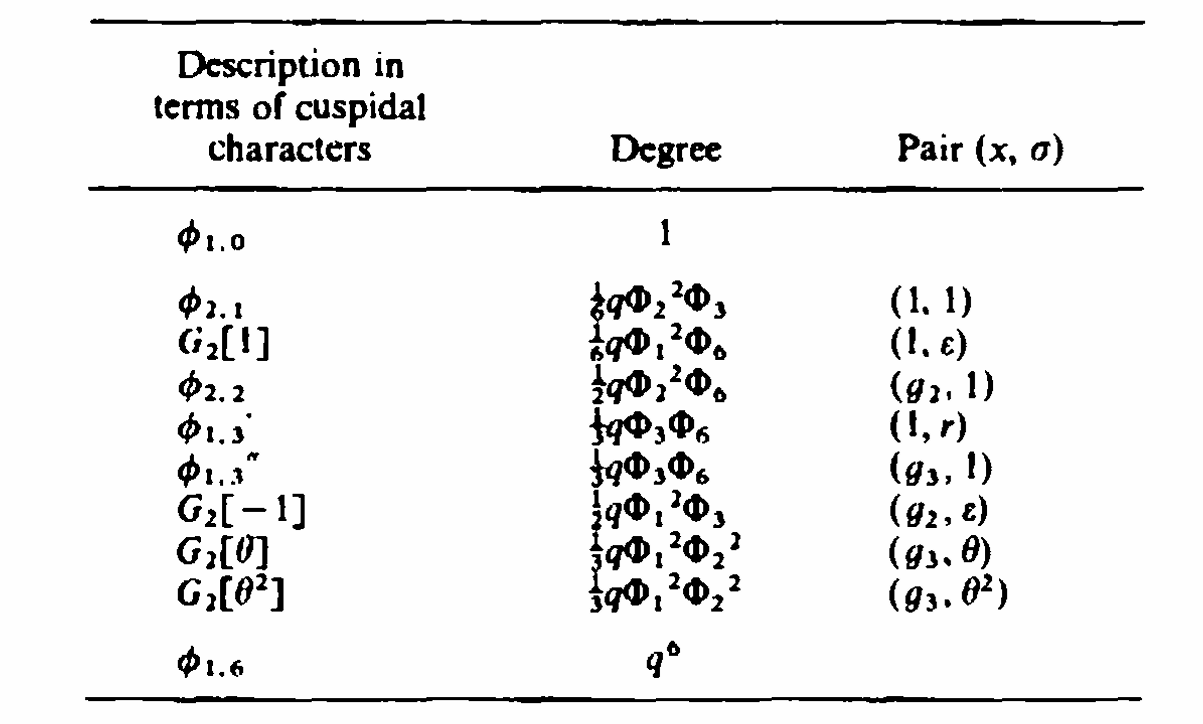
\includegraphics[width=0.8\textwidth]{cuspidals G_2.png}
    \end{center}
\end{example}

Finally, Lusztig defined a nonabelian Fourier transform on the set of irreducible characters of $G^F$. For each family $\mathcal{F}$ of unipotent characters parametrized by the group $\Gamma$, he considered the $|M(\Gamma)|\times|M(\Gamma)|$ matrix, whose $((x,\sigma),(y,\tau))$ entry is the value 
$$\{(x,\sigma),(y,\tau)\}=\frac{1}{|C_\Gamma(x)||C_\Gamma(y)|}\sum_{\substack{g\in \Gamma\\ xgyg^{-1}=gyg^{-1}x}}\sigma(gyg^{-1})\overline{\tau(g^{-1}xg)}.$$
Then he proved that this matrix is Hermitian and that it squares to the identity. It therefore induces an involution on the space $\CC[G^F]^{G^F}_\mathcal{F}$ of class functions spanned by the characters in $\mathcal{F}$, where we take the natural basis $\{\chi_{(x,\sigma)}^\mathcal{F}\ |\ (x,\sigma)\in M(\Gamma)\}$. Combining for each family, this gives an involution 
$$R:\CC_{un}[G^F]^{G^F}\longrightarrow \CC_{un}[G^F]^{G^F}$$
on the space $\CC_{un}[G^F]^{G^F}$ of class functions spanned by unipotent characters. This forces, for example, that $R(\chi_\phi)=R_\phi$ for all characters of $W$. The involution $R$ transforms unipotent characters into \textit{unipotent almost characters} that also satisfy the orthogonality relations and have a geometrical significance.

\begin{example}
    If $G^F$ is of type $A_l$, then the unipotent characters coincide with the almost characters.

    If $G^F$ is of type $G_2$, then $R$ fixes the characters $\phi_{1,0}$ and $\phi_{1,6}$ but transforms the third family according to the Fourier transform matrix
    \begin{center}
        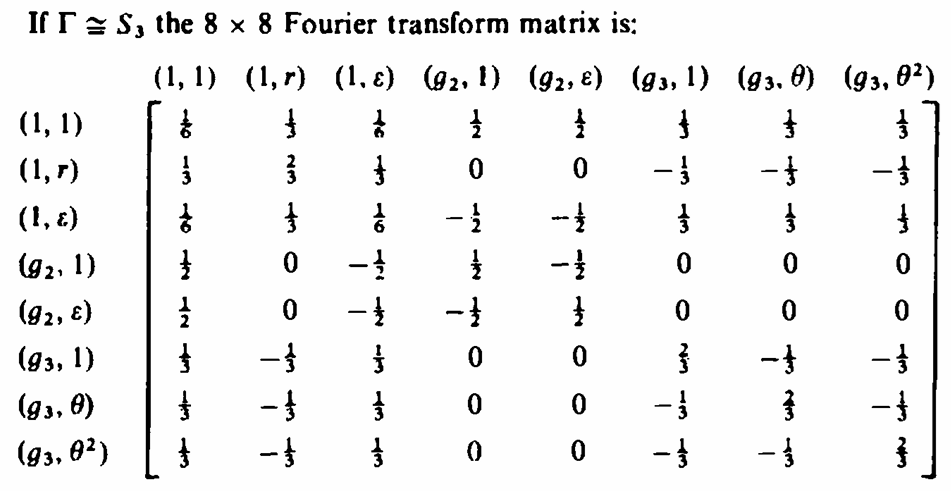
\includegraphics[width=0.8\textwidth]{Fourier matrix for S_3.png}
    \end{center}
\end{example}

The almost characters satisfy certain \textit{stability properties}. \textcolor{red}{Search what do they exactly mean by this.}
The aim of the next chapter is to discuss a lift of this map for $p$-adic groups.